% %\documentclass[russian,utf8,floatsection,equationsection,14pt]{eskdtext}
% \documentclass{article}
% 
% \usepackage[cp1251]{inputenc}  %% 1
% \usepackage[T2A]{fontenc}      %% 2
% \usepackage[russian]{babel}
% 
% % Better sans-serif fonts
% % \usepackage{pscyr}
% % \renewcommand{\rmdefault}{cmr}
% % \renewcommand{\sfdefault}{ftx}
% % \renewcommand{\ttdefault}{cmtt}
% % % Объявляем документ класса eskdtext (подробнее можно узнать из описания пакета
% % % eskdx) russian - текст на русском языке, utf8 - кодировка документа UTF-8
% % % floatsection - нумерация таблиц и рисунков с учётом номера главы,
% % % equationsection - то же для формул
% % \usepackage{longtable} % В документе используем пакет longtable для создания таблиц 
% % \usepackage{graphicx} %s Используем графику в документе
% % \usepackage{mathtext} % Русские буквы в формулах \usepackage[T2A]{fontenc}
% % \usepackage{setspace}
% % 
% % \ESKDdocName{Проект сети широкополосного доступа на базе FTTH в г. Тавда}
% % \ESKDsignature{ДИПЛОМНЫЙ ПРОЕКТ} 
% % \ESKDdepartment{%
% % Государственное образовательное учреждение высшего профессионального образования
% % }
% % \ESKDcompany{%
% % Сибирский государственный университет телекоммуникаций и информатики
% %  
% % (ГОУ ВПО СибГУТИ)
% % }
% % \ESKDauthor{Федотов~С.\,А.} % "Разраб." в штампе на листе содержания
% % \ESKDchecker{Иванов И.И.} % "Пров."  в штампе на листе содержания
% % \ESKDnormContr{Петров П.П.} % "Н. контр." в штампе на листе содержания
% % \ESKDapprovedBy{Сидоров С.С.}%  "Увт." в штампе на листе содержания
% % \ESKDdate{2013/05/02} % Дата (Год отображается на титульной странице)
% % \ESKDsignature{ФЗО 210406.052 ПЗ} % Шифр
% % \ESKDletter{}{У}{} % Литеры 
% % \renewcommand{\ESKDtheTitleFieldX}{
% % 	Новосибирск 
% % \ESKDtheYear~г.} % Шаблон для отображения в нижней части титульного листа города и года 
% % \ESKDtitleDesignedBy{Дипломник}{Федотов С.А.} % Подпись и дата под заголовком документа 
% % \ESKDtitleApprovedBy{Зав. Кафедрой}{Лебедянцев В.В.} % Утверждаю
% % \renewcommand{\baselinestretch}{1} % Задаём единичный межстрочный интервал 
% % \ESKDsectSkip{section}{5mm}{5mm}
% % \ESKDsectSkip{subsection}{5mm}{5mm}
% % \ESKDsectSkip{subsubsection}{5mm}{5mm}
% % \ESKDsectStyle{section}{\normalsize} % Заголовки глав обычным шрифтом
% % \ESKDsectStyle{subsection}{\normalsize} % Заголовки разделов обычным шрифтом
% % \ESKDsectStyle{subsubsection}{\normalsize} % Заголовки подразделов обычным шрифтом
% \date{\vspace{-5ex}}
% 
% \begin{document} % Маркер начала документа
% 
% \maketitle % Создать титульный лист на основе данных в заголовке
% % документа
% \tableofcontents % Создать содержание документа (потребуется дважды сформировать документ для того,
% % чтобы номера страниц сформировались правильно)
% \onehalfspacing
% % Начать следующий раздел с новой страницы
% \newpage 
\section*{Введение}
\addcontentsline{toc}{section}{Введение}
В настоящее время, люди страдающие серьезными системными заболеваниями
(например, сердечно-сосудистыми) стали получать возможность проходить необходимое лечение и даже возвращаться (до
определенной степени) к полноценной жизни. Основная трудность с которой они
сталкиваются при этом - необходимость постоянного врачебного наблюдения с целью
сохранения достигнутого состояния оздоровления. Наблюдение предполагает собой
частые визиты к врачу; отсюда вытекает потеря личного времени пациента на
преодоление расстояния, на ожидание в очереди и др. Помимо этого на медицинское
учреждение накладывается функция сбора и анализа медицинской статистики.

Согласно исследованиям GBI Research\footnote{ http://ria-ami.ru/news/26944 } в
ближайшие годы здравоохранение столкнется с серьезными проблемами: повысится
доля пожилых граждан в общей структуре населения и значительно увеличится
численность пациентов с хроническими заболеваниями — сердечно-сосудистыми,
легочными, а также диабетом. По оценкам Всемирного фонда диабета, к 2025 г. 80\%
пациентов с диабетом будут проживать в странах, где подавляющее число граждан
обладают низкими или средними доходами.

На основе полученных результатов очевидно возрастание необходимости в удаленном
медицинском обслуживании. Технические средства удаленного мониторинга, с одной
стороны, избавляют пациентов от необходимости регулярно посещать лечащих врачей
(что особенно важно для обитателей удаленных регионов), а с другой — на
регулярной основе обеспечивают медицинских работников актуальной информацией о
состоянии здоровья их подопечных.

После внимательного анализа приведенных выше фактов, стала прояснятся общая
проблема, присущая данному рода медицинского обслуживания. Пациенту для
соблюдения непрерывного медицинского наблюдения необходимо личное присутствие в
медицинском учреждении, даже в самых малозначимых ситуациях.
В то же время, последние  несколько лет возросли темпы компьтеризации населения,
также повсеместно стало  распространяться относительно недорогое подключение к
сети Интернет. В связи с этим становится вполне логичной идея частично
реализовать общение пациента и врача с использованием современных информационных
технологий.

Таким образом, основной целью разработки  является создание такой системы,
которая бы позволила реализовать обмен медицинской информацией между доктором и
пациентом дистанционно, через сеть Интернет. Система также должна хранить
полученную информацию и выполнять типовые операции с ними с целью мониторинга.
В целях исследования и разработки системы нами были использованы бизнес-процессы
и организационная структура медицинского учреждения “Кузбасский кардиологический
центр”.
% \newpage
\ESKDthisStyle{formII}
\section{Описание предприятия}
Кузбасский кардиологический центр представляет собой уникальный комплекс
специализированных научных и лечебно-профилактических учреждений, осуществляющих
высокотехнологичную медицинскую помощь пациентам с болезнями сердечно-сосудистой
системы.
\subsection{История предприятия}
История создания Кузбасского кардиологического центра началась в марте 1957
года, когда в Кемеровской области была сделана первая операция на сердце -
пальцевая митральная комиссуротомия при митральном стенозе. Операцию проводил
заслуженный врач РФ, почетный гражданин города Кемерово, хирург М.А.
Подгорбунский на базе отделения торакальной хирургии Областной клинической
больницы №1.

Год спустя, осенью 1958 года был организован кабинет для ангиокардиографии. В
1974 году на основании приказа МЗ СССР «Об организации центра
сердечно-сосудистой хирургии в г. Кемерово» на базе Областной клинической
больницы № 1 открыто кардиологическое отделение на 40 коек, а с 1975 года - на
50 коек.

В 1989 году Администрация города Кемерово принимает решение о строительстве
Кемеровского кардиологического  испансера (ККД) на правом берегу реки Томи в
живописном сосновом бору. Организация такого специализированного учреждения была
вызвана необходимостью расширения диагностических и лечебных возможностей
кардиологической помощи больным, страдающим сердечно-сосудистыми заболеваниями.
Возглавил кардиодиспансер доктор медицинских наук, профессор, в настоящее время
академик РАМН Леонид Семенович Барбараш, один из пионеров кардиохирургии
Кемеровской области. Созданию и развитию кардиодиспансера активно помогали
руководители крупных промышленных предприятий, администрации города и области.

С 1994 года управление учреждением осуществляется двумя руководителями:
генеральным директором Цыганковой Галиной Юсифовной и главным врачом Барбарашом
Леонидом Семёновичем.

К 1994 году в ККД создана основная диагностическая и лечебная база. Это
амбулаторная служба (многопрофильная районная и специализированная
кардиологическая поликлиника), диагностические отделения (функциональной
диагностики, ультразвуковых исследований, лучевой диагностики, клиническая
лаборатория и др.) и стационарные отделения (острой коронарной патологии, общей
кардиологии, реабилитационное отделение, отделения сердечно-сосудистой хирургии
и реанимации). В составе кардиодиспансера активно развивались хозрасчетные
структуры, мобильный кардиологический диспансер, гараж, гостиница и пр.
   
В этот же период началось развитие научно - производственной базы, открыты
экспериментальная лаборатория, производство биопротезов клапанов сердца и
сосудов. В 2001 году создается Государственное учреждение
«Научно-производственная проблемная лаборатория реконструктивной хирургии
сердца и сосудов Сибирского Отделения Российской академии медицинских наук»
(ГУ НППЛ РХСС СО РАМН).

В августе 2005 года введен в эксплуатацию 12-ти этажный госпитальный корпус ККД,
что увеличило количество стационарных коек с 142 до 172. Открылись отделение
детской кардиологии, неврологическое, нейрохирургическое, значительно
увеличились объемы работы отделений сердечно-сосудистой хирургии и
рентгенхирургических методов диагностики и лечения.

С 2006 года ККД становится главным звеном медицинского комплекса «Кузбасский
кардиологический центр» совместно с ГУ НППЛРХСС СО РАМН и производством
биопротезов (ЗАО «Неокор»), обеспечивающий единый технологический цикл оказания
помощи пациентам при сердечно-сосудистых заболеваниях. Центр стал базой кафедры
кардиологии и сердечно-сосудистой хирургии КемГМА.

В декабре 2008 года ГУ НППЛРХСС СО РАМН реорганизуется в
Научно-исследовательский институт комплексных проблем сердечно-сосудистых
заболеваний Сибирского отделения РАМН, с большим научным потенциалом и хорошей
лечебно-диагностической базой.

В 2010г. Кемеровская область вошла в федеральную программу "Совершенствование
оказания медицинской помощи больным с острой сосудистой патологией". В рамках
реализации этой программы создан 1 региональный сосудистый центр (РСЦ) и 3
первичных сосудистых центра (ПСО). Базой РСЦ стал МУЗ "ККД". РСЦ -
координирующий головной центр в  регионе, оказывающий высокотехнологичную помощь
больным с сосудистыми заболеваниями. Созданы отделения для лечения больных с
острым нарушением мозгового кровообращения и острым коронарным синдромом.
\section{Организационная структура предприятия}
На верхнем уровне декомпозиции в составе предприятия можно выделить следующие
группы работников:

\begin{enumerate}
\item врачебный состав; 
\item обслуживающий персонал; 
\item административная служба.
\end{enumerate}

Обслуживающий и административный персонал организован стандартным для
большинства государственных предприятий здравоохранения, поэтому не представляют
большого интереса для нашего исследования.
Наоборот лечебная деятельность Кузбасского Кардиоцентра (далее ККЦ) и будет
являться основной целью исследования организационной структуры предприятия.
Итак, основные подразделения предприятия. занимающиеся лечебной деятельностью,
можно отобразить на схеме.
\section{Основные подразделения предприятия}

\subsubsection{СО РАМН (ФГБУ "НИИ КПССЗ" СО РАМН)}
Учреждение (полное название “Научно - исследовательский институт комплексных
проблем сердечно-сосудистых заболеваний" ) создано с целью получения на основе
фундаментальных и прикладных исследований новых и углубления имеющихся знаний в
области  кардиологии, ангиологии и сердечно-сосудистой хирургии, направленных на
сохранение и укрепление здоровья человека, развитие здравоохранения и
медицинской науки, подготовку высококвалифицированных научных и медицинских
кадров.

Основные функции подразделения:
\begin{enumerate}
	\item проведение фундаментальных и прикладных исследований;
	\item разработка и апробация заменителей элементов сердечно-сосудистой системы
на основе биологических тканей, новых медицинских технологий лечения, 
диагностики и профилактики;
	\item осуществление медицинской деятельности.
\end{enumerate}

\subsubsection{Кемеровский Кардиологический Диспансер МБУЗ ККД}
Основные функции - предоставление населению медицинских услуг (лечения). В
составе подразделения находится множество отделов, среди которых можно выделить
поликлинику, научно-медицинские центры, а также стационар ККЦ, речь о котором
пойдет чуть ниже.

\subsubsection{Кафедра кардиологии}
Основные функции:  объединение терапевтических и хирургических аспектов
преподавания для обучения специалистов с комплексным подходом к ведению
пациентов с сердечно-сосудистой патологией.

\section{Подразделение связанное с предметной областью}

Поскольку цель нашей разработки является создание автоматизированой системы
мониторинга пациентов с ВПС, рассмотрим подразделение, которое занимается этим
вопросом.

Данным подразделением является Отделение детской кардиологии, которое входит в
состав Стационара ККЦ.

Центр детской кардиологии функционально объединяет стационарное и
поликлиническое звено. Основным направлением деятельности центра является
диагностика и подготовка к хирургическому лечению врождённых пороков сердца у
детей.

Для лечения детей с врождёнными пороками сердца  используются современные
методики:  выполнение  операций на открытом сердце в условиях искусственного
кровообращения  и эндоваскулярные малоинвазивные методики.

В ходе операций на открытом сердце устраняются врождённые пороки сердца с
преполнением малого круга кровообращения (дефект межжелудочковой перегородки,
дефект межпредсердной перегородки без чётких краёв, атриовентрикулярная
коммуникация), «синие» пороки (тетрада Фалло). Среди эндоваскулярных
вмешательств используются методики закрытия дефекта межпредсердной перегородки,
открытого артериального протока системой «Amplatzer».

В ходе работы центра постоянно происходит ротация врачебного персонала, что
позволяет наблюдать пациента с момента обращения в клинику и до момента оказания
хирургической коррекции, а так же осуществлять динамическое наблюдение в периоде
реабилитации.

Отделение рассчитано на 25 пациентов. Практическая работа осуществляется 10
сотрудниками. В штатах 4 врача детских-кардиологов, из которых 1 имеет высшую
категорию, 1 вторую квалификационную категорию, 6 медицинских сестёр, 3 с высшей
квалификационной категорией, 2 с первой.
% \newpage
\section{Существующие бизнес-процессы}

Для анализа предметной области выявим все процессы, связанные с лечением
пациентов с ВПС и отобразим их на IDEF0 диаграмме.

\subsubsection{Система мониторинга как процесс}

Входным объектом существующей в настоящее время системы мониторинга является сам
пациент. На выходе системы врачи выдают медицинское заключение о состоянии
здоровья пациента.

В процессе мониторинга в настоящее время используются всевозможные лабораторные
анализы, а также дневник наблюдения (который ведут родители или опекуны
пациента). В качестве оборудования также используются персональные компьютеры на
которых ведется база данных пациентов (представляет собой файл электронной
таблицы Excel). Следят за процессом мониторинга лица, назначqенные руководством
кардиоцентра и другие государственные служащие.

\subsubsection{Система мониторинга как совокупность процессов}

Как правило процесс мониторинга пациентов с ВПС (как и многие другие виды
лечений) начинается с предварительного приема. Прием проводится в учреждении
здравохранения по месту жительства - это позволяет к моменту приема
непосредственно в кардиоцентре  иметь некоторую медицинскую информацию
(результаты анализов, самостоятельные наблюдения пациента) и соответственно
разгрузить персонал и оборурдование ККЦ от большой входной нагрузки,
сконцетрировавашись на основной своей деятльности.

Во время врачебного приема родители пациента передают медицинскую информацию
(как правило это результаты наблюдения за его состоянием) словесно, а также  в
виде дневника наблюдения.

\subsubsection{Амбулаторный педиатрический прием}

Одним из трудоемким для обоих сторон процессов является периодический
амбулаторный прием по месту жительства.

Данный процесс состоит из 3 стадий. Сперва больной записывается на прием к
врачую. Во время записи родители пациента вносят записи о результатах своих
наблюдений. Далее больной приходит на прием к врачу. Врач по итогам осмотра
выдает заключение и направляет пациента на сдачу медицинскиха анализов. На
основаниии анализов либо проводится либо повторное обследование, либо выдается
расширенное направление на кардиобследование.

\subsubsection{Заключительная стадия мониторинга}

После кардиологического обследования пациента, врачи проводят анализ полученной
медицинской информации. На основании сделанных выводов врачи составляют
медицинское заключение и выдают рекомендации родителям и лечащим врачам. Данная
информация сообщается пациенту на заключительном осмотре.

% \newpage
\chapter{Проблемы}
В существующем бизнес-процессе существует ряд недостатков которые снижают
эффективность процесса лечения.

Процесс лечения и мониторинга детей с ВПС является достаточно длительным, сроки
измеряются годами. Обусловлен такой длительный период многими факторами,
рассмотрим основные из них.

\subsection{Задержка с операционным вмешательством}
Лечение врожденного порока сердца возможно только с помощью операционного
вмешательства, которое может задерживаться. Основной причиной задержки является
денежный вопрос, потому что операции детей с ВПС достаточно дорогостоящие
(средняя стоимость открытой операции на сердце — 236 000 рублей\footnote{
http://www.pomogi.org/projects/heart }).
Важно вести постоянный контроль за состоянием пациента в дооперационный период.

\subsection{Наблюдение в послеоперационный период}
Наблюдение в послеоперационный период очень важно из-за рисков осложнений и
возможности повторных операционных вмешательств.

\subsection{Расстояние}
Не в каждом городе есть специализированная клиника для лечения детей с ВПС.
Из-за задержки с операцией необходимо либо переезжать в другой город для того
чтобы лечащий врач мог контролировать состояние ребенка, либо периодически
приезжать на осмотр. Тот и другой способы достаточно затратны, и к тому же могут
негативно сказаться на состоянии ребенка.

\subsection{Взаимодействие}
В дооперационный и послеоперационный перид наблюдение за состоянием ребенка
ведет как правило кардиолог по месту жительства, а операцию проводит уже другой
врач-хирург. Как правило хирург и кардиолог непосредственно не контактируют друг
с другом. Предоставление возможностей общаться и делиться информацией о пациенте
в между хирургом и кардиологом в процессе лечения позитивно скажется на процессе
реабилитации и лечения.

\subsection{Анализ, прогнозирование, тенденции}
Выше было сказано что процесс лечения достаточно длителен. Важно хранить всю
историю лечения в одном месте с возможностью простого доступа к ней.

\subsection{Лечение в стационаре}
Длительное пребывание пациента в стационаре снижает его социальные навыки -
ребенок остается без общения со сверстниками, много времени проводит внутри
помещения, затрудняется активное времяпрепровождение (если оно возможно). Также
происходит отрыв ребенка от образовательного процеса, что очень влияет на его
дальнейшие жизненные достижения. В связи с этим, важно свести реабилитационный
период к минимуму.

% \newpage
\chapter{Цели}
\subsection{Постоянный мониторинг состояния пациента	}

Постоянный мониторинг позволит получать наиболее актуальную информацию о
состоянии пациента в процессе лечения и во время реабилитационного периода. Так
же важно организовать ненавязчивый мониторинг в течении повседневной жизни
пациента. Рассмотрим основные направления мониторинга которые будут охвачены в
системе.

\subsubsection{Амбулаторное наблюдение}

Система должна позволять пациентам в добровольном порядке и в ненавязчивой форме
предоставлять данные осостоянии своего здоровья. Так как данные будут приходить
в систему из внешних незашищенных источников - необходимо обечпечивать
максимальную защищенность каналов передачи данных.

\subsubsection{Наблюдение в стационаре}

Необходимо организовать круглосуточное наблюдение за больными, помещенными в
специально оборудованное медицинское учреждение. В систему должны поступать
данные:

\begin{enumerate}
	\item с медицинских устройств;
	\item данные по результатам обследования;
	\item данные по результатам приемов и обходов.
\end{enumerate}

\subsubsection{Постоянный анализ получаемых данных}

Недостаточно просто хранить все данные в процессе лечения и возлагать
ответственность за их обработку на врача. Необходимо организовать обработку
данных в автоматическом режиме. Это позволит снизить нагрузку на врача и
повысить его эффективность в процессе лечения.
Реализация автоматическо обработки диагностических данных - достаточно сложный
процесс, поэтому ограничимся следующими направлениями в анализе данных:

\begin{enumerate}
	\item оценка эффективности лечения:
		\begin{enumerate}
			\item оценка влияния лекарственных препаратов;
			\item оценка влияния процедур.
		\end{enumerate}
	\item полный жизненный цикл процесса лечения.
\end{enumerate}

\subsubsection{Постоянное взаимодействие пациента с врачом}

Для повышения эффективности лечения пациента необходимо снизить издержки со
стороны пациента и врача на процесс общения и ибмена информации между ними.
Основным видом взаимодействия пациента и врача является личный прием у врача.
Такая форма взаимодействия наиболее эффективна и привычна с социальной и
профессиональных точек зрения, но она не всегда приемлима. В некоторых ситуация,
когда доктору или пациенту важно лишь уточнить некторые детали, лучше
организовать более простую форму взаимодействия между ними. Упрощенными формами
личного приема у врача могут являться:

\begin{enumerate}
  	\item интернет-прием - процесс представляющий из себя обычный прием у врача
организованный по средстам сети Интернет;
	\item  online-консльтация - процесс получения
унтересующих пациента сведений у специалиста в определенной области или
консультанта.
\end{enumerate}
 
Введение даных видов взаимодействия позволит в значительной мере сократить
нагрузку на врача и снизить временные и денежные издержки для пациента.

\subsubsection{Взаимодействие между врачами}

В процессе лечения пациента принимает участие широкий круг специалистов. Каждый
специалист должен иметь возможность получить в кратчайщие сроки информацию о:

\begin{enumerate}
	\item текущем состоянии пациента;
	\item заключениях других докторов;
	\item обследованиях и лекарстенных препаратах назначенных пациенту.
\end{enumerate}

Своевременное получение актуальной информации позволит более эффективно
организовать процесс лечения, за счет снижения временных затрат как пациента,
так и доктора.

% \newpage
\section{Принципиальные требования}
\subsection{Данные}
\subparagraph{Все в одном месте.}
Система должна обеспечивать доступность всех необходимых данных для лечащего
врача. Данная возможность позволит сократить время приема у врача и количество
приемов, т.к. связующим звеном между врачами станет не пациент с карточкой, а
система с набором всех данных необходимы для принятия дальнейщи решений по
процессу лечения.

Данные к которым система должна обеспечивать непосредственный доступ:

\begin{enumerate}
  \item данные о пациенте:
  \begin{enumerate}
    \item данные обследований;
    \item назначенное лечение;
    \item самочувствие;
    \item расписание приемов;
    \item расписание операций.
  \end{enumerate}
  \item справочные данные:
  \begin{enumerate}
    \item справочники;
    \item законодальные акты;
    \item словари.
  \end{enumerate}
  \item данные о системе:
  \begin{enumerate}
    \item очереди на прием;
    \item очереди на обследование;
    \item наличие лекарственных препаратов;
    \item наличие оборудования.
  \end{enumerate}     
\end{enumerate}





\subsection{Интерфейс}
\subparagraph{Эргономичность.}

Интуитивный интерфейс должен обеспечивать простое взаимоействие с системой без
организации специальной учебной программы по пользованию системой для врача и
пациента. 

Независимость от устройств с помощью которых врач иили пациент получают
доступ к системе.

\section{Требования к системе}

\subsubsection{Надежность}
\subparagraph{Поддержка целостности данных.}
Данные о пациенте будут хранится достаточно долгий промежуток времени в течении которого важно обеспечивать целостность данных. Под целостностью данных прежде всего понимаются:

\begin{enumerate}
  \item после поступления в систему данных из внешних систем, данные не должны
  менять своего состояния;
  \item целостность связей между данными. 
\end{enumerate}

\subparagraph{Резервирование основных узлов системы.}
Важно обеспечить доступность системы даже при отказе одного из узлов. Данное
qтребование может быть выполнено за счет дублирование основных узлов системы,
или распределения нагрузоки между однотипными узлами.

\subsubsection{Безопасность}
\subparagraph{Защита персональных данных больного.}

В соответствии с Законом № 152-ФЗ персональными данными является любая
информация, связанная с физическим лицом (субъектом персональных данных),
позволяющая идентифицировать конкретное физическое лицо среди прочих лиц. В
персональных данных физического лица выделяют общие и специальные категории.
Согласно данному закону, персональные данные это любая информация, относящаяся к
определенному или определяемому на основании такой информации физическому лицу
(субъекту персональных данных), в том числе его фамилия, имя, отчество, год,
месяц, дата и место рождения, адрес, семейное, социальное, имущественное
положение, образование, профессия, доходы, другая информация.
Среди конфиденциальной информации можно выделить медицинскую (или врачебную)
тайну. Российское законодательство определяет врачебную тайну как «информацию о
факте обращения за медицинской помощью, состоянии здоровья гражданина, диагнозе
его заболевания и иные сведения, полученные при его обследовании и лечении».
Фактически, на текущий момент защита личных данных в медицинских информационных
системах представлена  двумя базовыми аспектами.
Первым из них является этический (профессиональный) аспект взаимодействия врача
и пациента, который регулируется нормами врачебной этики и законом о защите
личных данных пациентов.
Второй аспект представляет собой защиту информации в медицинской системе с
технической точки зрения, то есть, здесь речь идет о создании адекватных
механизмов защиты данных непосредственно в рамках программно-аппаратного
комплекса информационной системы.
По мнению экспертов Фрайбургского университета (Германия), до 60\%\footnote{
	http://www.cnews.ru/reviews/free/national2006/articles/datasecure/
} утечек
медицинской информации происходит из-за действий медицинских работников, причем,
не только лечащих или консультирующих врачей, но и обслуживающего и
административного персонала медучреждений. Только 40\% утечек информации
происходит по техническим причинам — в результате взломов информационных систем
злоумышленниками, хищения баз данных и персональных компьютеров.

\subsubsection{Доступность}
\subparagraph{Доступность на чтение.}
Система должна быть доступна на чтение с любого устройства поддерживающего
доступ к сети интернет.
\subparagraph{Доступность на запись.}
Доступность ситемы на запись должна ограничиваться на уровне распределения прав
доступа к системе согласно ролям пользователей.

\subsubsection{Масштабируемость}
Масштабируемость - возможность системы справляться с возрастающими нагрузками за
счет модернизации системы. Важно понимать что масштабируемость должна
обеспечивать модернизацию системы с минимальными изменениями.

\subsubsection{Гибкость}
\subparagraph{Простота модернизации.}
Данное требование включает в себя как простоту обновления существующих
компонентов так и максимально быструю возможность расширения системы.

Обновление компонентов системы не должно быть критичным. Система должна
поддерживать так называемое “обновление на лету”. В идеале время неработоспособности системы при обновлении должно стремится к нулю.

Расширение функционала системы не должно приводить к существенной переработке
существующего фугкционала.

\subparagraph{Минимум зависимостей.}
Любая информационная система состоит из большого числа компонентов. Важно чтобы
связи между компонентами были минимальны. Выполение данного условия позволит
сделать систему более независисмой от конкретных технологий и технических
решений.
\section{Требования к технологиям}
Надежность - способность системы сохранять работоспособность при нормальных
условиях эксплуатации.

Доступность - возможность свободного (разумеется, при наличии необходимых прав
доступа к системе) получения требуемой услуги 

Актуальность - соответствие
функциональности системы современным требованиям предполагаемой целевой
аудитории 

Поддержка - необходима дистанционная поддержка пользователей по
вопросам возникшим в результате работы системы. Данное требование должно быть
обязательно к исполнению в контексте предметной области (некоторые медицинские
процессы не требуют отлагательства). Также желательна возможность относительно
оперативного добавления или изменения текущего функционала системы.

Открытость - открытый доступ к системе, заключающийся в соблюдении
международных и национальных стандартов в области используемых информационных
технологий с целью свободного взаимодействия  программных приложений, данных,
персонала и пользователей системы.

Низкая стоимость - при исполнении данного требования желательно использование
программного обеспечения с открытым исходным кодом. Аппаратное обеспечение
должно без проблем поддерживать озвученные выше требования к системе, поэтому
для снижения расходов предпочтительно привлечение спонсоров.

Функциональность (специфика бизнеса, стратегические приоритеты, географическая
распределенность и т.д.)

% \end{document} % Маркер завершения документа

\documentclass[a4paper,14pt]{extreport} %размер бумаги устанавливаем А4, шрифт
% 12пунктов
\usepackage{extsizes}
\usepackage{cmap} % для кодировки шрифтов в pdf
\usepackage[T2A]{fontenc}
\usepackage[utf8]{inputenc}
\usepackage[russian]{babel}
\usepackage{hyperref}
\hypersetup{
    colorlinks,
    citecolor=black,
    filecolor=black,
    linkcolor=black,
    urlcolor=black
}

\usepackage{graphics}
\ifx\pdfoutput\undefined
\usepackage{graphicx}
\else
\usepackage[pdftex]{graphicx}
\fi
\graphicspath{{images/}}

\usepackage{amssymb,amsfonts,amsmath,amsthm} % математические дополнения от АМС
\usepackage{indentfirst} % отделять первую строку раздела абзацным отступом тоже
\usepackage[usenames,dvipsnames]{color} % названия цветов
\usepackage{makecell}
\usepackage{multirow} % улучшенное форматирование таблиц
\usepackage{ulem} % подчеркивания
\usepackage[dvipsnames]{xcolor}

\usepackage{listings}
\renewcommand\lstlistingname{Листинг}
\renewcommand\lstlistlistingname{Листинг}
\lstloadlanguages{Ruby}
\lstset{
    xleftmargin=\parindent,
	breaklines=true,
	basicstyle=\ttfamily\color{black},
	commentstyle = \ttfamily\color{red},
	keywordstyle=\ttfamily\color{blue},
	stringstyle=\color{orange},
	numberstyle=\tiny,
	xleftmargin=0.1cm,
	numbersep=5pt,
	columns=flexible
	keepspaces=true,
	captionpos=b
}
 
\linespread{1.3} % полуторный интервал
\renewcommand{\rmdefault}{ftm} % Times New Roman
\frenchspacing

\usepackage{fancyhdr}
\pagestyle{fancy}
\fancyhf{}
\fancyhead[R]{\thepage}
\fancyheadoffset{0mm}
\fancyfootoffset{0mm}
\setlength{\headheight}{17pt}
\renewcommand{\headrulewidth}{0pt}
\renewcommand{\footrulewidth}{0pt}
\fancypagestyle{plain}{ 
    \fancyhf{}
    \rhead{\thepage}}

\usepackage{titlesec}
 
\titleformat{\chapter}[display]
    {\filcenter}
    {\MakeUppercase{\chaptertitlename} \thechapter}
    {8pt}
    {\bfseries}{}
 
\titleformat{\section}
    {\normalsize\bfseries}
    {\thesection}
    {1em}{}
 
\titleformat{\subsection}
    {\normalsize\bfseries}
    {\thesubsection}
    {1em}{}
 
% Настройка вертикальных и горизонтальных отступов
\titlespacing*{\chapter}{0pt}{-30pt}{8pt}
\titlespacing*{\section}{\parindent}{*4}{*4}
\titlespacing*{\subsection}{\parindent}{*4}{*4}

\usepackage{geometry}
\geometry{left=3cm}
\geometry{right=1.5cm}
\geometry{top=2.4cm}
\geometry{bottom=2.4cm}

\usepackage{enumitem}
\makeatletter
    \AddEnumerateCounter{\asbuk}{\@asbuk}{м)}
\makeatother
\setlist{nolistsep}
\renewcommand{\labelitemi}{-}
\renewcommand{\labelenumi}{\asbuk{enumi})}
\renewcommand{\labelenumii}{\arabic{enumii})}

\newcommand{\empline}{\mbox{}\newline}
\newcommand{\likechapterheading}[1]{ 
    \begin{center}
    \textbf{\MakeUppercase{#1}}
    \end{center}
    \empline}
    
\makeatletter
    \renewcommand{\@dotsep}{2}
    \newcommand{\l@likechapter}[2]{{\bfseries\@dottedtocline{0}{0pt}{0pt}{#1}{#2}}}
\makeatother
\newcommand{\likechapter}[1]{    
    \likechapterheading{#1}    
    \addcontentsline{toc}{likechapter}{\MakeUppercase{#1}}}

\usepackage{tocloft}
\renewcommand{\cfttoctitlefont}{\hspace{0.38\textwidth} \bfseries\MakeUppercase}
\renewcommand{\cftbeforetoctitleskip}{-1em}
\renewcommand{\cftchapfont}{\normalsize\bfseries \MakeUppercase{\chaptername} }
\renewcommand{\cftsecfont}{\hspace{0pt}}
\renewcommand{\cftsubsecfont}{\hspace{-10pt}}
\renewcommand{\cftbeforechapskip}{1em}
\renewcommand{\cftparskip}{-1mm}
\renewcommand{\cftdotsep}{1}
\setcounter{tocdepth}{2} % задать глубину оглавления — до subsection включительно

\begin{document}
\tableofcontents % это оглавление, которое генерируется автоматически
\newpage 
\section*{Введение}
\addcontentsline{toc}{section}{Введение}
В настоящее время, люди страдающие серьезными системными заболеваниями
(например, сердечно-сосудистыми) стали получать возможность проходить необходимое лечение и даже возвращаться (до
определенной степени) к полноценной жизни. Основная трудность с которой они
сталкиваются при этом - необходимость постоянного врачебного наблюдения с целью
сохранения достигнутого состояния оздоровления. Наблюдение предполагает собой
частые визиты к врачу; отсюда вытекает потеря личного времени пациента на
преодоление расстояния, на ожидание в очереди и др. Помимо этого на медицинское
учреждение накладывается функция сбора и анализа медицинской статистики.

Согласно исследованиям GBI Research\footnote{ http://ria-ami.ru/news/26944 } в
ближайшие годы здравоохранение столкнется с серьезными проблемами: повысится
доля пожилых граждан в общей структуре населения и значительно увеличится
численность пациентов с хроническими заболеваниями — сердечно-сосудистыми,
легочными, а также диабетом. По оценкам Всемирного фонда диабета, к 2025 г. 80\%
пациентов с диабетом будут проживать в странах, где подавляющее число граждан
обладают низкими или средними доходами.

На основе полученных результатов очевидно возрастание необходимости в удаленном
медицинском обслуживании. Технические средства удаленного мониторинга, с одной
стороны, избавляют пациентов от необходимости регулярно посещать лечащих врачей
(что особенно важно для обитателей удаленных регионов), а с другой — на
регулярной основе обеспечивают медицинских работников актуальной информацией о
состоянии здоровья их подопечных.

После внимательного анализа приведенных выше фактов, стала прояснятся общая
проблема, присущая данному рода медицинского обслуживания. Пациенту для
соблюдения непрерывного медицинского наблюдения необходимо личное присутствие в
медицинском учреждении, даже в самых малозначимых ситуациях.
В то же время, последние  несколько лет возросли темпы компьтеризации населения,
также повсеместно стало  распространяться относительно недорогое подключение к
сети Интернет. В связи с этим становится вполне логичной идея частично
реализовать общение пациента и врача с использованием современных информационных
технологий.

Таким образом, основной целью разработки  является создание такой системы,
которая бы позволила реализовать обмен медицинской информацией между доктором и
пациентом дистанционно, через сеть Интернет. Система также должна хранить
полученную информацию и выполнять типовые операции с ними с целью мониторинга.
В целях исследования и разработки системы нами были использованы бизнес-процессы
и организационная структура медицинского учреждения “Кузбасский кардиологический
центр”.
\newpage
\ESKDthisStyle{formII}
\section{Описание предприятия}
Кузбасский кардиологический центр представляет собой уникальный комплекс
специализированных научных и лечебно-профилактических учреждений, осуществляющих
высокотехнологичную медицинскую помощь пациентам с болезнями сердечно-сосудистой
системы.
\subsection{История предприятия}
История создания Кузбасского кардиологического центра началась в марте 1957
года, когда в Кемеровской области была сделана первая операция на сердце -
пальцевая митральная комиссуротомия при митральном стенозе. Операцию проводил
заслуженный врач РФ, почетный гражданин города Кемерово, хирург М.А.
Подгорбунский на базе отделения торакальной хирургии Областной клинической
больницы №1.

Год спустя, осенью 1958 года был организован кабинет для ангиокардиографии. В
1974 году на основании приказа МЗ СССР «Об организации центра
сердечно-сосудистой хирургии в г. Кемерово» на базе Областной клинической
больницы № 1 открыто кардиологическое отделение на 40 коек, а с 1975 года - на
50 коек.

В 1989 году Администрация города Кемерово принимает решение о строительстве
Кемеровского кардиологического  испансера (ККД) на правом берегу реки Томи в
живописном сосновом бору. Организация такого специализированного учреждения была
вызвана необходимостью расширения диагностических и лечебных возможностей
кардиологической помощи больным, страдающим сердечно-сосудистыми заболеваниями.
Возглавил кардиодиспансер доктор медицинских наук, профессор, в настоящее время
академик РАМН Леонид Семенович Барбараш, один из пионеров кардиохирургии
Кемеровской области. Созданию и развитию кардиодиспансера активно помогали
руководители крупных промышленных предприятий, администрации города и области.

С 1994 года управление учреждением осуществляется двумя руководителями:
генеральным директором Цыганковой Галиной Юсифовной и главным врачом Барбарашом
Леонидом Семёновичем.

К 1994 году в ККД создана основная диагностическая и лечебная база. Это
амбулаторная служба (многопрофильная районная и специализированная
кардиологическая поликлиника), диагностические отделения (функциональной
диагностики, ультразвуковых исследований, лучевой диагностики, клиническая
лаборатория и др.) и стационарные отделения (острой коронарной патологии, общей
кардиологии, реабилитационное отделение, отделения сердечно-сосудистой хирургии
и реанимации). В составе кардиодиспансера активно развивались хозрасчетные
структуры, мобильный кардиологический диспансер, гараж, гостиница и пр.
   
В этот же период началось развитие научно - производственной базы, открыты
экспериментальная лаборатория, производство биопротезов клапанов сердца и
сосудов. В 2001 году создается Государственное учреждение
«Научно-производственная проблемная лаборатория реконструктивной хирургии
сердца и сосудов Сибирского Отделения Российской академии медицинских наук»
(ГУ НППЛ РХСС СО РАМН).

В августе 2005 года введен в эксплуатацию 12-ти этажный госпитальный корпус ККД,
что увеличило количество стационарных коек с 142 до 172. Открылись отделение
детской кардиологии, неврологическое, нейрохирургическое, значительно
увеличились объемы работы отделений сердечно-сосудистой хирургии и
рентгенхирургических методов диагностики и лечения.

С 2006 года ККД становится главным звеном медицинского комплекса «Кузбасский
кардиологический центр» совместно с ГУ НППЛРХСС СО РАМН и производством
биопротезов (ЗАО «Неокор»), обеспечивающий единый технологический цикл оказания
помощи пациентам при сердечно-сосудистых заболеваниях. Центр стал базой кафедры
кардиологии и сердечно-сосудистой хирургии КемГМА.

В декабре 2008 года ГУ НППЛРХСС СО РАМН реорганизуется в
Научно-исследовательский институт комплексных проблем сердечно-сосудистых
заболеваний Сибирского отделения РАМН, с большим научным потенциалом и хорошей
лечебно-диагностической базой.

В 2010г. Кемеровская область вошла в федеральную программу "Совершенствование
оказания медицинской помощи больным с острой сосудистой патологией". В рамках
реализации этой программы создан 1 региональный сосудистый центр (РСЦ) и 3
первичных сосудистых центра (ПСО). Базой РСЦ стал МУЗ "ККД". РСЦ -
координирующий головной центр в  регионе, оказывающий высокотехнологичную помощь
больным с сосудистыми заболеваниями. Созданы отделения для лечения больных с
острым нарушением мозгового кровообращения и острым коронарным синдромом.
\section{Организационная структура предприятия}
На верхнем уровне декомпозиции в составе предприятия можно выделить следующие
группы работников:

\begin{enumerate}
\item врачебный состав; 
\item обслуживающий персонал; 
\item административная служба.
\end{enumerate}

Обслуживающий и административный персонал организован стандартным для
большинства государственных предприятий здравоохранения, поэтому не представляют
большого интереса для нашего исследования.
Наоборот лечебная деятельность Кузбасского Кардиоцентра (далее ККЦ) и будет
являться основной целью исследования организационной структуры предприятия.
Итак, основные подразделения предприятия. занимающиеся лечебной деятельностью,
можно отобразить на схеме.
\section{Основные подразделения предприятия}

\subsubsection{СО РАМН (ФГБУ "НИИ КПССЗ" СО РАМН)}
Учреждение (полное название “Научно - исследовательский институт комплексных
проблем сердечно-сосудистых заболеваний" ) создано с целью получения на основе
фундаментальных и прикладных исследований новых и углубления имеющихся знаний в
области  кардиологии, ангиологии и сердечно-сосудистой хирургии, направленных на
сохранение и укрепление здоровья человека, развитие здравоохранения и
медицинской науки, подготовку высококвалифицированных научных и медицинских
кадров.

Основные функции подразделения:
\begin{enumerate}
	\item проведение фундаментальных и прикладных исследований;
	\item разработка и апробация заменителей элементов сердечно-сосудистой системы
на основе биологических тканей, новых медицинских технологий лечения, 
диагностики и профилактики;
	\item осуществление медицинской деятельности.
\end{enumerate}

\subsubsection{Кемеровский Кардиологический Диспансер МБУЗ ККД}
Основные функции - предоставление населению медицинских услуг (лечения). В
составе подразделения находится множество отделов, среди которых можно выделить
поликлинику, научно-медицинские центры, а также стационар ККЦ, речь о котором
пойдет чуть ниже.

\subsubsection{Кафедра кардиологии}
Основные функции:  объединение терапевтических и хирургических аспектов
преподавания для обучения специалистов с комплексным подходом к ведению
пациентов с сердечно-сосудистой патологией.

\section{Подразделение связанное с предметной областью}

Поскольку цель нашей разработки является создание автоматизированой системы
мониторинга пациентов с ВПС, рассмотрим подразделение, которое занимается этим
вопросом.

Данным подразделением является Отделение детской кардиологии, которое входит в
состав Стационара ККЦ.

Центр детской кардиологии функционально объединяет стационарное и
поликлиническое звено. Основным направлением деятельности центра является
диагностика и подготовка к хирургическому лечению врождённых пороков сердца у
детей.

Для лечения детей с врождёнными пороками сердца  используются современные
методики:  выполнение  операций на открытом сердце в условиях искусственного
кровообращения  и эндоваскулярные малоинвазивные методики.

В ходе операций на открытом сердце устраняются врождённые пороки сердца с
преполнением малого круга кровообращения (дефект межжелудочковой перегородки,
дефект межпредсердной перегородки без чётких краёв, атриовентрикулярная
коммуникация), «синие» пороки (тетрада Фалло). Среди эндоваскулярных
вмешательств используются методики закрытия дефекта межпредсердной перегородки,
открытого артериального протока системой «Amplatzer».

В ходе работы центра постоянно происходит ротация врачебного персонала, что
позволяет наблюдать пациента с момента обращения в клинику и до момента оказания
хирургической коррекции, а так же осуществлять динамическое наблюдение в периоде
реабилитации.

Отделение рассчитано на 25 пациентов. Практическая работа осуществляется 10
сотрудниками. В штатах 4 врача детских-кардиологов, из которых 1 имеет высшую
категорию, 1 вторую квалификационную категорию, 6 медицинских сестёр, 3 с высшей
квалификационной категорией, 2 с первой.
\newpage
\section{Существующие бизнес-процессы}

Для анализа предметной области выявим все процессы, связанные с лечением
пациентов с ВПС и отобразим их на IDEF0 диаграмме.

\subsubsection{Система мониторинга как процесс}

Входным объектом существующей в настоящее время системы мониторинга является сам
пациент. На выходе системы врачи выдают медицинское заключение о состоянии
здоровья пациента.

В процессе мониторинга в настоящее время используются всевозможные лабораторные
анализы, а также дневник наблюдения (который ведут родители или опекуны
пациента). В качестве оборудования также используются персональные компьютеры на
которых ведется база данных пациентов (представляет собой файл электронной
таблицы Excel). Следят за процессом мониторинга лица, назначqенные руководством
кардиоцентра и другие государственные служащие.

\subsubsection{Система мониторинга как совокупность процессов}

Как правило процесс мониторинга пациентов с ВПС (как и многие другие виды
лечений) начинается с предварительного приема. Прием проводится в учреждении
здравохранения по месту жительства - это позволяет к моменту приема
непосредственно в кардиоцентре  иметь некоторую медицинскую информацию
(результаты анализов, самостоятельные наблюдения пациента) и соответственно
разгрузить персонал и оборурдование ККЦ от большой входной нагрузки,
сконцетрировавашись на основной своей деятльности.

Во время врачебного приема родители пациента передают медицинскую информацию
(как правило это результаты наблюдения за его состоянием) словесно, а также  в
виде дневника наблюдения.

\subsubsection{Амбулаторный педиатрический прием}

Одним из трудоемким для обоих сторон процессов является периодический
амбулаторный прием по месту жительства.

Данный процесс состоит из 3 стадий. Сперва больной записывается на прием к
врачую. Во время записи родители пациента вносят записи о результатах своих
наблюдений. Далее больной приходит на прием к врачу. Врач по итогам осмотра
выдает заключение и направляет пациента на сдачу медицинскиха анализов. На
основаниии анализов либо проводится либо повторное обследование, либо выдается
расширенное направление на кардиобследование.

\subsubsection{Заключительная стадия мониторинга}

После кардиологического обследования пациента, врачи проводят анализ полученной
медицинской информации. На основании сделанных выводов врачи составляют
медицинское заключение и выдают рекомендации родителям и лечащим врачам. Данная
информация сообщается пациенту на заключительном осмотре.

\newpage
\chapter{Проблемы}
В существующем бизнес-процессе существует ряд недостатков которые снижают
эффективность процесса лечения.

Процесс лечения и мониторинга детей с ВПС является достаточно длительным, сроки
измеряются годами. Обусловлен такой длительный период многими факторами,
рассмотрим основные из них.

\subsection{Задержка с операционным вмешательством}
Лечение врожденного порока сердца возможно только с помощью операционного
вмешательства, которое может задерживаться. Основной причиной задержки является
денежный вопрос, потому что операции детей с ВПС достаточно дорогостоящие
(средняя стоимость открытой операции на сердце — 236 000 рублей\footnote{
http://www.pomogi.org/projects/heart }).
Важно вести постоянный контроль за состоянием пациента в дооперационный период.

\subsection{Наблюдение в послеоперационный период}
Наблюдение в послеоперационный период очень важно из-за рисков осложнений и
возможности повторных операционных вмешательств.

\subsection{Расстояние}
Не в каждом городе есть специализированная клиника для лечения детей с ВПС.
Из-за задержки с операцией необходимо либо переезжать в другой город для того
чтобы лечащий врач мог контролировать состояние ребенка, либо периодически
приезжать на осмотр. Тот и другой способы достаточно затратны, и к тому же могут
негативно сказаться на состоянии ребенка.

\subsection{Взаимодействие}
В дооперационный и послеоперационный перид наблюдение за состоянием ребенка
ведет как правило кардиолог по месту жительства, а операцию проводит уже другой
врач-хирург. Как правило хирург и кардиолог непосредственно не контактируют друг
с другом. Предоставление возможностей общаться и делиться информацией о пациенте
в между хирургом и кардиологом в процессе лечения позитивно скажется на процессе
реабилитации и лечения.

\subsection{Анализ, прогнозирование, тенденции}
Выше было сказано что процесс лечения достаточно длителен. Важно хранить всю
историю лечения в одном месте с возможностью простого доступа к ней.

\subsection{Лечение в стационаре}
Длительное пребывание пациента в стационаре снижает его социальные навыки -
ребенок остается без общения со сверстниками, много времени проводит внутри
помещения, затрудняется активное времяпрепровождение (если оно возможно). Также
происходит отрыв ребенка от образовательного процеса, что очень влияет на его
дальнейшие жизненные достижения. В связи с этим, важно свести реабилитационный
период к минимуму.

\newpage
\chapter{Цели}
\subsection{Постоянный мониторинг состояния пациента	}

Постоянный мониторинг позволит получать наиболее актуальную информацию о
состоянии пациента в процессе лечения и во время реабилитационного периода. Так
же важно организовать ненавязчивый мониторинг в течении повседневной жизни
пациента. Рассмотрим основные направления мониторинга которые будут охвачены в
системе.

\subsubsection{Амбулаторное наблюдение}

Система должна позволять пациентам в добровольном порядке и в ненавязчивой форме
предоставлять данные осостоянии своего здоровья. Так как данные будут приходить
в систему из внешних незашищенных источников - необходимо обечпечивать
максимальную защищенность каналов передачи данных.

\subsubsection{Наблюдение в стационаре}

Необходимо организовать круглосуточное наблюдение за больными, помещенными в
специально оборудованное медицинское учреждение. В систему должны поступать
данные:

\begin{enumerate}
	\item с медицинских устройств;
	\item данные по результатам обследования;
	\item данные по результатам приемов и обходов.
\end{enumerate}

\subsubsection{Постоянный анализ получаемых данных}

Недостаточно просто хранить все данные в процессе лечения и возлагать
ответственность за их обработку на врача. Необходимо организовать обработку
данных в автоматическом режиме. Это позволит снизить нагрузку на врача и
повысить его эффективность в процессе лечения.
Реализация автоматическо обработки диагностических данных - достаточно сложный
процесс, поэтому ограничимся следующими направлениями в анализе данных:

\begin{enumerate}
	\item оценка эффективности лечения:
		\begin{enumerate}
			\item оценка влияния лекарственных препаратов;
			\item оценка влияния процедур.
		\end{enumerate}
	\item полный жизненный цикл процесса лечения.
\end{enumerate}

\subsubsection{Постоянное взаимодействие пациента с врачом}

Для повышения эффективности лечения пациента необходимо снизить издержки со
стороны пациента и врача на процесс общения и ибмена информации между ними.
Основным видом взаимодействия пациента и врача является личный прием у врача.
Такая форма взаимодействия наиболее эффективна и привычна с социальной и
профессиональных точек зрения, но она не всегда приемлима. В некоторых ситуация,
когда доктору или пациенту важно лишь уточнить некторые детали, лучше
организовать более простую форму взаимодействия между ними. Упрощенными формами
личного приема у врача могут являться:

\begin{enumerate}
  	\item интернет-прием - процесс представляющий из себя обычный прием у врача
организованный по средстам сети Интернет;
	\item  online-консльтация - процесс получения
унтересующих пациента сведений у специалиста в определенной области или
консультанта.
\end{enumerate}
 
Введение даных видов взаимодействия позволит в значительной мере сократить
нагрузку на врача и снизить временные и денежные издержки для пациента.

\subsubsection{Взаимодействие между врачами}

В процессе лечения пациента принимает участие широкий круг специалистов. Каждый
специалист должен иметь возможность получить в кратчайщие сроки информацию о:

\begin{enumerate}
	\item текущем состоянии пациента;
	\item заключениях других докторов;
	\item обследованиях и лекарстенных препаратах назначенных пациенту.
\end{enumerate}

Своевременное получение актуальной информации позволит более эффективно
организовать процесс лечения, за счет снижения временных затрат как пациента,
так и доктора.

\newpage
\section{Принципиальные требования}
\subsection{Данные}
\subparagraph{Все в одном месте.}
Система должна обеспечивать доступность всех необходимых данных для лечащего
врача. Данная возможность позволит сократить время приема у врача и количество
приемов, т.к. связующим звеном между врачами станет не пациент с карточкой, а
система с набором всех данных необходимы для принятия дальнейщи решений по
процессу лечения.

Данные к которым система должна обеспечивать непосредственный доступ:

\begin{enumerate}
  \item данные о пациенте:
  \begin{enumerate}
    \item данные обследований;
    \item назначенное лечение;
    \item самочувствие;
    \item расписание приемов;
    \item расписание операций.
  \end{enumerate}
  \item справочные данные:
  \begin{enumerate}
    \item справочники;
    \item законодальные акты;
    \item словари.
  \end{enumerate}
  \item данные о системе:
  \begin{enumerate}
    \item очереди на прием;
    \item очереди на обследование;
    \item наличие лекарственных препаратов;
    \item наличие оборудования.
  \end{enumerate}     
\end{enumerate}





\subsection{Интерфейс}
\subparagraph{Эргономичность.}

Интуитивный интерфейс должен обеспечивать простое взаимоействие с системой без
организации специальной учебной программы по пользованию системой для врача и
пациента. 

Независимость от устройств с помощью которых врач иили пациент получают
доступ к системе.

\section{Требования к системе}

\subsubsection{Надежность}
\subparagraph{Поддержка целостности данных.}
Данные о пациенте будут хранится достаточно долгий промежуток времени в течении которого важно обеспечивать целостность данных. Под целостностью данных прежде всего понимаются:

\begin{enumerate}
  \item после поступления в систему данных из внешних систем, данные не должны
  менять своего состояния;
  \item целостность связей между данными. 
\end{enumerate}

\subparagraph{Резервирование основных узлов системы.}
Важно обеспечить доступность системы даже при отказе одного из узлов. Данное
qтребование может быть выполнено за счет дублирование основных узлов системы,
или распределения нагрузоки между однотипными узлами.

\subsubsection{Безопасность}
\subparagraph{Защита персональных данных больного.}

В соответствии с Законом № 152-ФЗ персональными данными является любая
информация, связанная с физическим лицом (субъектом персональных данных),
позволяющая идентифицировать конкретное физическое лицо среди прочих лиц. В
персональных данных физического лица выделяют общие и специальные категории.
Согласно данному закону, персональные данные это любая информация, относящаяся к
определенному или определяемому на основании такой информации физическому лицу
(субъекту персональных данных), в том числе его фамилия, имя, отчество, год,
месяц, дата и место рождения, адрес, семейное, социальное, имущественное
положение, образование, профессия, доходы, другая информация.
Среди конфиденциальной информации можно выделить медицинскую (или врачебную)
тайну. Российское законодательство определяет врачебную тайну как «информацию о
факте обращения за медицинской помощью, состоянии здоровья гражданина, диагнозе
его заболевания и иные сведения, полученные при его обследовании и лечении».
Фактически, на текущий момент защита личных данных в медицинских информационных
системах представлена  двумя базовыми аспектами.
Первым из них является этический (профессиональный) аспект взаимодействия врача
и пациента, который регулируется нормами врачебной этики и законом о защите
личных данных пациентов.
Второй аспект представляет собой защиту информации в медицинской системе с
технической точки зрения, то есть, здесь речь идет о создании адекватных
механизмов защиты данных непосредственно в рамках программно-аппаратного
комплекса информационной системы.
По мнению экспертов Фрайбургского университета (Германия), до 60\%\footnote{
	http://www.cnews.ru/reviews/free/national2006/articles/datasecure/
} утечек
медицинской информации происходит из-за действий медицинских работников, причем,
не только лечащих или консультирующих врачей, но и обслуживающего и
административного персонала медучреждений. Только 40\% утечек информации
происходит по техническим причинам — в результате взломов информационных систем
злоумышленниками, хищения баз данных и персональных компьютеров.

\subsubsection{Доступность}
\subparagraph{Доступность на чтение.}
Система должна быть доступна на чтение с любого устройства поддерживающего
доступ к сети интернет.
\subparagraph{Доступность на запись.}
Доступность ситемы на запись должна ограничиваться на уровне распределения прав
доступа к системе согласно ролям пользователей.

\subsubsection{Масштабируемость}
Масштабируемость - возможность системы справляться с возрастающими нагрузками за
счет модернизации системы. Важно понимать что масштабируемость должна
обеспечивать модернизацию системы с минимальными изменениями.

\subsubsection{Гибкость}
\subparagraph{Простота модернизации.}
Данное требование включает в себя как простоту обновления существующих
компонентов так и максимально быструю возможность расширения системы.

Обновление компонентов системы не должно быть критичным. Система должна
поддерживать так называемое “обновление на лету”. В идеале время неработоспособности системы при обновлении должно стремится к нулю.

Расширение функционала системы не должно приводить к существенной переработке
существующего фугкционала.

\subparagraph{Минимум зависимостей.}
Любая информационная система состоит из большого числа компонентов. Важно чтобы
связи между компонентами были минимальны. Выполение данного условия позволит
сделать систему более независисмой от конкретных технологий и технических
решений.
\section{Требования к технологиям}
Надежность - способность системы сохранять работоспособность при нормальных
условиях эксплуатации.

Доступность - возможность свободного (разумеется, при наличии необходимых прав
доступа к системе) получения требуемой услуги 

Актуальность - соответствие
функциональности системы современным требованиям предполагаемой целевой
аудитории 

Поддержка - необходима дистанционная поддержка пользователей по
вопросам возникшим в результате работы системы. Данное требование должно быть
обязательно к исполнению в контексте предметной области (некоторые медицинские
процессы не требуют отлагательства). Также желательна возможность относительно
оперативного добавления или изменения текущего функционала системы.

Открытость - открытый доступ к системе, заключающийся в соблюдении
международных и национальных стандартов в области используемых информационных
технологий с целью свободного взаимодействия  программных приложений, данных,
персонала и пользователей системы.

Низкая стоимость - при исполнении данного требования желательно использование
программного обеспечения с открытым исходным кодом. Аппаратное обеспечение
должно без проблем поддерживать озвученные выше требования к системе, поэтому
для снижения расходов предпочтительно привлечение спонсоров.

Функциональность (специфика бизнеса, стратегические приоритеты, географическая
распределенность и т.д.)

\newpage
\ESKDthisStyle{formII}
\section{Готовые решения}
Тема разработки программного обеспечения и информационных систем для медицинских
учреждений в последнее время получила большое распространение. Многие
разработчики решают начать делать свой так называемый “стартап”, также часто
можно встретить предложения от ИТ-компаний.

Существующие решения можно разделить на несколько основных классов.

\subsection{Решения на базе системы 1С:Предприятие}
\subsubsection{1С Медицина Поликлиника}
Данное решение\footnote{
	\url{http://www.v8.1c.ru/solutions/product.jsp?prod_id=149}
} 
предназначено для автоматизации деятельности медицинских
организаций различных организационно-правовых форм, оказывающих медицинскую
помощь в амбулаторно-поликлинических условиях. Программный продукт служит для
ведения взаиморасчетов с контрагентами, управления потоками пациентов,
персонифицированного учета оказанной медицинской помощи.

\subsubsection{1С Рарус Амбулатория}
Данный продукт\footnote{http://rarus.ru/press/publications/126187/} комплексно
автоматизирует деятельность медицинского учреждения.
Помимо глубоко реализованной системы автоматизации документооборота, хотелось бы
отметить характерное для мира 1С систем наличие реестров и справочников
служебной медицинской информации, например, Банк Стволовых Клеток «КриоЦентр».

\subsection{Решения для автоматизации медицинского документооборота}
Комплексная медицинская информационная система (КМИС). Уменьшает затраты доктора
на ведение документации связанной с приемом пациентов, выдачей направлений и
т.д.
Медицинская информационная система AKSi-офис\footnote{
	\url{http://www.aksimed.ru/products/aksi_line/AKSi-Office.php}
} 
(на базе системы Microsoft Office).
Программное обеспечение от фирмы ТрастМед - аналогичный функционал.

\subsection{Комплексная автоматизация медицинского предприятия}
В первую очередь хотелось бы отметить отечественную разработку - Медицинская
информационная система AKSi-клиника от АКСИМЕД. Среди ее основных функций
хотелось бы отметить следующие:

\begin{enumerate}
  \item комплексная автоматизация всех процессов наблюдения, диагностики и
  лечения амбулаторных и стационарных пациентов;
  \item эффективное управление персоналом, ресурсами и
  финансово-\\экономической деятельностью ЛПУ, автоматизация
  медико-\\статистического контроля и планирования;
  \item однократный ввод информации в электронную историю болезни (электронную
  медицинскую карту) пациента с последующим многократным использованием этих сведений и поддержкой принятия врачебных решений;
  \item сквозная компьютеризация работы регистратуры, поликлиники, стационара,
  отделения скорой медицинской помощи, стоматологических кабинетов и других подразделений ЛПУ;
  \item обеспечение безопасности персональных данных в соответствии с
  Федеральным законом от 27 июля 2006 г. № 152-ФЗ.
\end{enumerate}

Также существуют множество зарубежных решений. Среди них можно упомянуть систему
разработанную и используемую в США - Practicefusion, чей девиз “Больше пациентов
- меньше работы”.

\subsection{Выбор готового решения}
Среди всех рассмотренных выше систем можно выявить общую тенденцию - ИТ-компании
предлагают в первую очередь автоматизацию медицинского документооборота.
Некоторые системы предлагают анализ и диагностику, но она заточена под широкое
использование.

Разработанная нами система позволяет решить поставленные в начале исследования
проблемы, а именно автоматизированный дистанционный (с определенной степенью)
сбор медицинской информации, мониторинг (проведение какого-либо анализа над
собранными), позволяет проводить коммуникацию между пациентами.

Разумеется озвученные нами возможности реализованы в существующих ныне системах
в том или ином виде. Здесь нужно отметить, что рассмотренные выше программные
средства и системы стоят больших денег и медицинское учреждение может сэкономить
внедряя нашу систему именно на том что наш система реализует конкретные
возможности (необходимые прежде всего для лечения больных с ВПС), а не внедряя
большой пакет возможностей, многие из которых могут никогда не пригодится.

Кроме того использование широко тиражированного программного обеспечения может
поставить в зависимость от решений фирмы-разработчика, что может оказать
нежелательным для предприятия со столь ответственной деятельностью. Наша же
система готова к дальнейшим изменениям потенциального заказчика, так
разрабатывается скорее для конкретных учреждений, а не для массовой реализации.
\newpage
\section{Корректировка безнес-процессов}
Рассмотрим процесс мониторинга в контексте будущей системы.

\subsection{Составляющие процесса мониторинга}

Единственным объектом исследования в системе является - обследуемый пациент. Система должна вести постоянный мониторинг и анализ состояния пациента.
Для получения данных о пациенте и их анализа могут быть использованы:

\begin{enumerate}
  \item Медицинские устройства. К ним относится аппараты, расположенны в
  лечебном учреждении и находящиеся в общем доступе для всех пациентов. К ним можно отнести рентген-установка, МРТ-сканер, УЗИ, тонометры, термометры, пульсметры и другие.
  \item Персональные устройства мониторинга. К ним можности приборы, доступные
  для использованиии в домашних условиях, а именно: электронные тонометры и термометры. Помимио этих приборов существуют так называемы комплексные датчики предназначеные для пользователей, не являющихся специалистами в области сердечно-сосудистой диагностики. К таким приборам относится Ангиоскан-01М (Персональная версия) – предназначен для работы под управлением персонального компьютера. Данный прибор надевается на палец пациента и устанавливает подключение к персональному компьтеру или ноутбуку. Прибор позволяет измерять следуюущие показатели: частоты сердечных сокращений; жесткости сосудов; типа пульсовой волны; биологического возраста сосудов; индекса сатурации (насыщение гемоглобина кислородом); уровня стресса.
  \item Сервер с необходимым програмным обеспечением. На нем будет развернута
  база данных, в которой будут храниться персональные данные всех участников системы,медицинская информация пациентов и прочие информационные объекты, котоыре будут определын ниже,  в разделе Концептуальная модель предметной области. Также на сервере будет находиться веб-интерфейс системы, доступный пользовтаелям.
\end{enumerate}

Процесс мониторинга должен соответствовать определенным стандартам и законодательным актам.

Контролировать процесс должен лечащий врач или врач, непосредственно, осуществяющий оказание той или иной услуги пациенту.

Результаты процесса мониторинга представляются в виде различного рода отчетов.

\subsection{Основные этапы процесса мониторинга}

\subsubsection{Регистрация в системе}

Этап предназначен для создания учетной записи пациента при обращении в данное
лечщее учреждение впервые. С данной учетной записью будут соотносится данные,
полученные в процессе лечения, обследований. Важно чтобы продолжительность
данного этапа была минимальной, а процедура регистрации максимально простой,
чтобы процесс обследования пациента начался максимально быстро.
Возможны два варианта регистрации пациента в системе:

\begin{enumerate}
  \item Самостоятельная регистрация. Данный вариант подходит для иногородних
  пациентов.
  \item Регистрация при посещении лечащего учреждения.
\end{enumerate}

После прохождения процедуры регистрации пациент может быть записан на первичный
прием к врачу.

\subsubsection{Первичное обследование}

На первичном приеме врач формирует электронную карту обследований, которые
необходимо пройти пациенту для оценки состояния здоровья. Факторами влияющими на
набор обследований который должен пройти пациент являются:
\begin{enumerate}
  \item Устные показания пациента
  \item Больничная карта пациента
  \item Опыт врача   
\end{enumerate}

Во время первичного приема у врача начинается непостредственный постоянный
мониторинг за состоянием пациента.

После составления карты обследования пациент проходит первичное обследование.
Первичное обследование необходимо для формализации состояния пациента на момент
обращения в лечащее учреждение. Оценка состояния пациента, полученная в
результате первичного обследования будет учитываться в показателях оценки
эффективности лечения.

\subsubsection{Лечение}
После прохождения пациентом первичного обследования формируется план лечения
пациента. План лечения пациента может быть многоэтапным. После завершения
каждого этапа происходит оценка эффективности лечения.

План лечения на каждом этапе может включать в себя:

\begin{enumerate}
  \item Режим дня пациента
  \item Режим приема лекарственных препаратов
  \item Расписание приемов
  \item Расписание обследований    
\end{enumerate}

Основной задачей системы на данном этапе является ослеживание качественных и
количественных показателей состояния пациента.

\subsubsection{Мониторинг}
Процесс мониторинга является “сквозным” и присутствут на многих этапах. Основной
задачей процесса является сбор данных в процессе лечения и обследований
пациента.
Основными процессами в результате которых в систему попадают данные о пациенте
являются:

\begin{enumerate}
  \item Прием у врача
  \item Стационарное лечение
  \item Обследования
  \item Амбулаторное лечение 
\end{enumerate}

Основными источниками даных о пациенте являются:

\begin{enumerate}
  \item Результаты обследований
  \item Результаты анализов
  \item Результаты осмотров у врача
  \item Устные показания пациента
  \item Показания врача 
\end{enumerate}

Основные способы внесения данных в систему:

\begin{enumerate}
  \item Ручной ввод
  \begin{enumerate}
    \item Ввод данных пациентом
    \item Ввод данных врачом
  \end{enumerate}
  \item Автоматический ввод данных медицинскими устройствами
\end{enumerate}

\subsubsection{Накопление данных}
Процесс заключается в сохранении поступающих в систему данных для их последующей
обработки и анализа.

\subsubsection{Анализ данных}
Объем данных, поступающих в систему достаточно большой. Для ускорения обработки
данных их необходимо анализировать. Согласно требованиям к системе, процесс
анализа данных включает в себя:

\begin{enumerate}
  \item Оценку эффективности лечения
  \begin{enumerate}
    \item Оценки влияния лекарственных препаратов
    \item Оценки влияния процедур, операций 
  \end{enumerate}
  \item Получение отчетов. Отчеты представлены в виде:
  \begin{enumerate}
    \item Агрегированные данные
    \item Рекомендации по лечению
  \end{enumerate}  
\end{enumerate}











\newpage
\section{Анализ предметной области}
\subsection{Концептуальная модель предметной области}

Определим основные объекты предметной области и выясним отношения между ними.

\subsubsection{Пациент}
Сущность отражает личную информацию о реальном пациенте.

Атрибуты:
\begin{enumerate}
  \item паспортные данные;
  \item номер полиса;
  \item номер личной больничной карты\footnote{
  	Сложно будет перевести сразу все учреждение на электронные больничные карты
  	поэтому некоторое время обычная больничная карта и электронная будут
  	сущестовать параллельно.
  };
  \item контактные данные.
\end{enumerate}

\subsubsection{Врач}
Сущность отражает данные о реальном докторе.

Атрибуты:
\begin{enumerate}
  \item паспортные данные;
  \item контактные данные;
  \item профессиональные данные; 
\end{enumerate}

\subsubsection{Менеджер}
Сущность отражает человека контролирующего работу системы.

Атрибуты:
\begin{enumerate}
  \item паспортные данные;
  \item контактные данные;
  \item профессиональные данные.   
\end{enumerate}

\subsubsection{Диагноз}
Сущность отражает реальный диагноз согласно “Международной статистической
классификации болезней и проблем, связанных со здоровьем” (ICD 10).

Атрибуты:
\begin{enumerate}
  \item класс диагноза;
  \item название диагноза.   
\end{enumerate}

\subsubsection{Лекарство}
Сущность отражает реальное лекарственный препарат.

Атрибуты:
\begin{enumerate}
  \item название лекарства;
  \item побочные эффекты;
  \item время приема;
  \item дозы;
  \item порядок приема. 
\end{enumerate}

\subsubsection{Обследование}
Сущность отражает реальное обследование доступное пациентам лечащего учреждения
в процессе лечения.

Атрибуты:
\begin{enumerate}
  \item суть обследования; 
  \item дата обследования; 
  \item результат обследования. 
\end{enumerate}

 \subsubsection{Прием}
Сущность отражает реальный прием у врача. Так как система должна иметь
возможноть сопровождать два типа приема: обычный и интернет прием, необходимо
чтобы набор атрибутов у них был максимально одинаковым. Выполнение данного
условия облегчит перевод учреждения на электронный прием.
 
Атрибуты
\begin{enumerate}
  \item дата приема; 
  \item результат приема; 
  \item данные сопровождающие прием. 
\end{enumerate}

\subsection{Связи между объектами предметной области}
Выявленные объекты предметной области, не покрывают всех функциональных
требований к системе и не учитывают технических реализаций и алгоритмов
построения информационных систем.

\subsection{Уточненние объектов предметной области}
Объекты “Врач”, “Пациент” и “Менеджер” имеют общий набор атрибутов, который
логично вынести в отдельный объект родитель “Пользователь”. Данный шаг упростит
процедуры регистрации, авторизации и процесс контроля прав доступа к системе,
так как необходимо будет контролировать только один объект вместо трех.

Объекты “Прием” и “Обследование” - это некоторые события. Логичным будет
выделить отдельный объект родитель - “Событие”. “Событие” будет связано с
пользователем через объект “Календарь” - отражающий определенный этап лечения.
Каждое событие имеет “Результат”. Событие может быть повторяющимся (прием
лекарственного препарата 3 раза в день). 

Лекарственные препараты и диагнозы являются справочниками, которые логичным
будет наследовать от объекта родителя “Справочник”.

“Справочник” и “Электронная карта” - это документы. Для облегчения работы с ними
логичным будет ввести объект родитель “Документ”.
 
 
\newpage
\chapter{Структура системы}
Под структурой системы будем понимать совокупность элементов, составляющих
систему, и связи между ними. Ниже рассмотрим основные компоненты системы.
Деление в контексте структуры достаточно условное, но оно позволит разграничить
области ответственности каждого компонента системы. Разграничение
ответственностей позволит упростить структуру системы и снизить связанность
элементов системы. Каждая из подсистем должна соответствовать требованиям к
системе приведенным выше.

\subsection{Подсистема ввода данных}
Подсистема ввода данных должна соответствовать требованию “доступности на
запись” и обеспечивать слудующие возможности:

\begin{enumerate}
  \item Ручной ввод данных - непосредственно участниками системы, доктором,
  пациентом, менеджером.
  \item Автоматический ввод данных - получение данных с различных устройств
  диагностики состояния пациента.
  \item Проверка вводимых данных на корректность. Корректность данных
  определяется исходя из контекста использования данных и типа данных.
  \item Абстракция. Доступ к источнику данных должен быть через легкозаменяемую
  абстракцию. Это позволит не зависеть от конкретного поставщика и выполнить требование “гибкости”.
\end{enumerate}

\subsection{Подсистема доступа к данным}
Подсистема доступа к данным должна соответствовать требованию “доступности на
чтение” и обеспечивать уровень абстракции от источника данных чтобы
соответствовать требованию “гибкости”. Так же должен обеспечиваться доступ как
для внешних, так и для внутренних потребителей.

\subsection{Подсистема хранения данных}
Подсистемма хранения данных должна обеспечивать:
\begin{enumerate}
  \item Целостность данных
  \item Возможность управления доступом к данным
  \item Возможности ускорения доступа к данным
  \item Возможность компенсировать увелчение нагрузки
\end{enumerate}
Обязательными являются требования к “надежности”, “безопасности” и
“масштабируемости”.

\subsection{Подсистема анализа данных}
Подсистема анализа данных должна обеспечивать возможность анализа данных,
поступающих из подсистемы ввода данных. Доступ к данным осуществляется через
подсистему доступа к данным. Промежуточные результаты работы могут сохранятся в
подсистеме хранения данных.
Результаты работы подсистемы анализа данных должны быть представлены в виде двух
видов отчетов:

\begin{enumerate}
  \item Отчет по запросу
  \item Автоматический отчет
\end{enumerate}

\subsection{Подсистема управления доступом}
Подсистема управления доступом должна:
\begin{enumerate}
  \item Обеспечивать возможность контроля доступа к данным в зависисмости от роли пользователя в системе.
  \item Реагировать на попытки несанкционированного доступа к данным.
\end{enumerate}

\newpage
\chapter{Проектирование}
Выше были выделены основные компоненты системы и разграничены функции и
ответственность между ними. Теперь необходимо определиться с конкретной
реализацией выбранных компонентов и со схемой взаимодействия между ними. 
Общая архитектура системы представлена на рисунке
\ref{ris:general_architecture}. Нижу будут рассмотрены основные компоненты
и описаны их назначения.

\begin{figure}[h]
\center{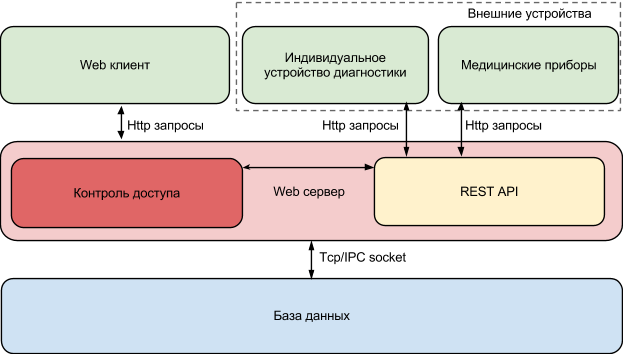
\includegraphics[width=1\linewidth]{general_architecture.eps}}
\caption{Общая архитектура системы.}
\label{ris:general_architecture}
\end{figure}

\subsection{Web клиент}
Клиент разделяет функции подсистемы ввода данных и подсистемы доступа к данным.
Основной задачей клиента является предоставление доступа к системе пользователям
с помощью веб-браузера или другого программного обеспечения способного работать
с протоколом HTTP. С точки зрения требования доступности, реализация в виде web
клиента наиболее оптимальна, так как веб-браузеры есть на всех современных
платформах и устройствах.

\subsection{Web сервер}
Основной задачей Web сервера является - организация взаимодействия между
различными клиентами и системой хранения данных. Также в рамках Web сервера
будут реализованы:
\begin{enumerate}
  \item бизнес-логика системы;
  \item контроль доступа к системе;
  \item подсистема унифицированного доступа к системе хранения данных;
  \item подсистема анализа данных;
  \item REST API для унифицированного взаимодействия с внешними источниками и
потребителями данных.
\end{enumerate}

\subsection{REST API}
Основной задачей является предоставление публичного интерфейса для ввода данных
с внешних источников.

\subsection{База данных}
Достаточно долгое время основным типом системы хранения данных была SQL база
данных. Однако в последние годы получает распространение NoSQL системы хранения.
Данные подходы к организации источника данных преследуют одну цель - обеспечить
долговременное, надежное хранение структурированных данных. Каждый подход имеет
свои преимущества и недостатки.
Для того чтобы определится какого типа будет система хранения данных необходимо
сформировать требования к системе, а затем на основании требований выбрать
наиболее подходящий тип системы.

\subsubsection{Требования к системе хранения данных}
Надежность - очень широкое понятие в терминах баз данных. Рассмотрим основные
составляющие надежной системы хранения.
\subparagraph{Обеспечение целостности данных.}
SQL системы изначально проектировались чтобы соответствовать основным принципам
ACID и как следствие предоставляют возможность хранить данные в нормализованном
виде, явно определяя связи между элементами базы даных. Однако такой подход
несет дополнительную нагрузку на базу данных, т.к. необходимо констролировать
целостность данных а базе.
NoSQL решения изначально проектировались как полная альтернатива SQL решениям.
Они позволяют хранить данные в максимально денормализованном виде. При таком
подходе вся ответственность за целостность даных возлагается целиком на
разработчиков.
\subparagraph{Масштабируемость.} 
При росте числа пользователей базы данных возникает проблема обработки большого
числа запросов к базе данных. Данную проблему можно решить за счет
горизонтальной или вертикальной масштабируемости ситемы.

При вертикальной масштабируемости предлагается обновлять конфигурацию сервера на
более современную для повышения производительности. При таком подходе очевидно
что общая производительность ситемы, если не брать в счет програмную
составляющую, ограничивается только прогресом в области производства аппаратного
обеспечения. Как правило местом преткновения становится скорость операций i/o на
жестком диске. Также стоит учитывать что цены на новинки всегда завышены и
нецелесообразно будет платить достаточно крупные суммы за повышение
производительности на несколько процентов.

При горизонтальном масштабировании предлагается распределять нагрузку на
несколько серверов баз данных. При таком подходе не нужно покупать новое
дорогостоящее оборудование, производительность не упирается в скорость i/o
операций на жестком диске, а производительность системы повышается
прямопропорционально числу серверов. Достаточно обеспечить необходимое
количество серверов чтобы балансировать нагрузку между ними.
На самом деле на этом вопрос масштабируемости не ограничивается, т.к. необходимо
учитывать еще один важный фактор - размер базы данных. Некоторые современные
базы данных поддерживают механизм партицирования. Данный механизм позволяет
разбивать таблицу на несколько частей. В результате чего возможно хранить данные
на разных носителях. Данный механиз повышает скорость доступа к данным за счет
того что выборка манипуляции с даными происходят не в контексте всей таблицы а в
контексте конкретной части таблицы. Не стоит забывать и о выборе файловой
системы под файлы базы данных и драйвера который будет управлять распределением
данных в файловой системе.
\subparagraph{Быстродействие.} 

Скорость работы подсистемы хранения данных непосредственно влияет на
продолжительность приема. Важно чтобы доступ к данным был максимально быстрым.

SQL решение накладывает некоторые ограничения. Прежде всего это индексы и
транзакции, которые могут заметно снизить скорость вставки данных, но без них
может значительно снижаться скорость выбрки данных.

NoSQL решение потенциально не имеет проблем со вставкой данных. Теоретически
вставка данных должна происходить со скоростью равной скорости записи в
оперативную память. Стоит отметить что все современные SQL базы данных
производят первичную запись данных так же в оперативную память.

\subparagraph{Выбор между SQL и NoSQL.}
Выбор между двумя подходами достаточно сложная задача. В рамках выбранной
предметной области система может быть спроектирована как NoSQL так и SQL
подходом. Однако SQL подход обеспечивает большую согласованность данных и более
простую реализацию. Так же немаловажным фактором в пользу SQL подхода является
наличие более развитых средств разработки.



\end{document}